% Native editable composition from verified, unchanged IDE images.
\par
\begin{figure}[htbp]
  \centering
  \sbox0{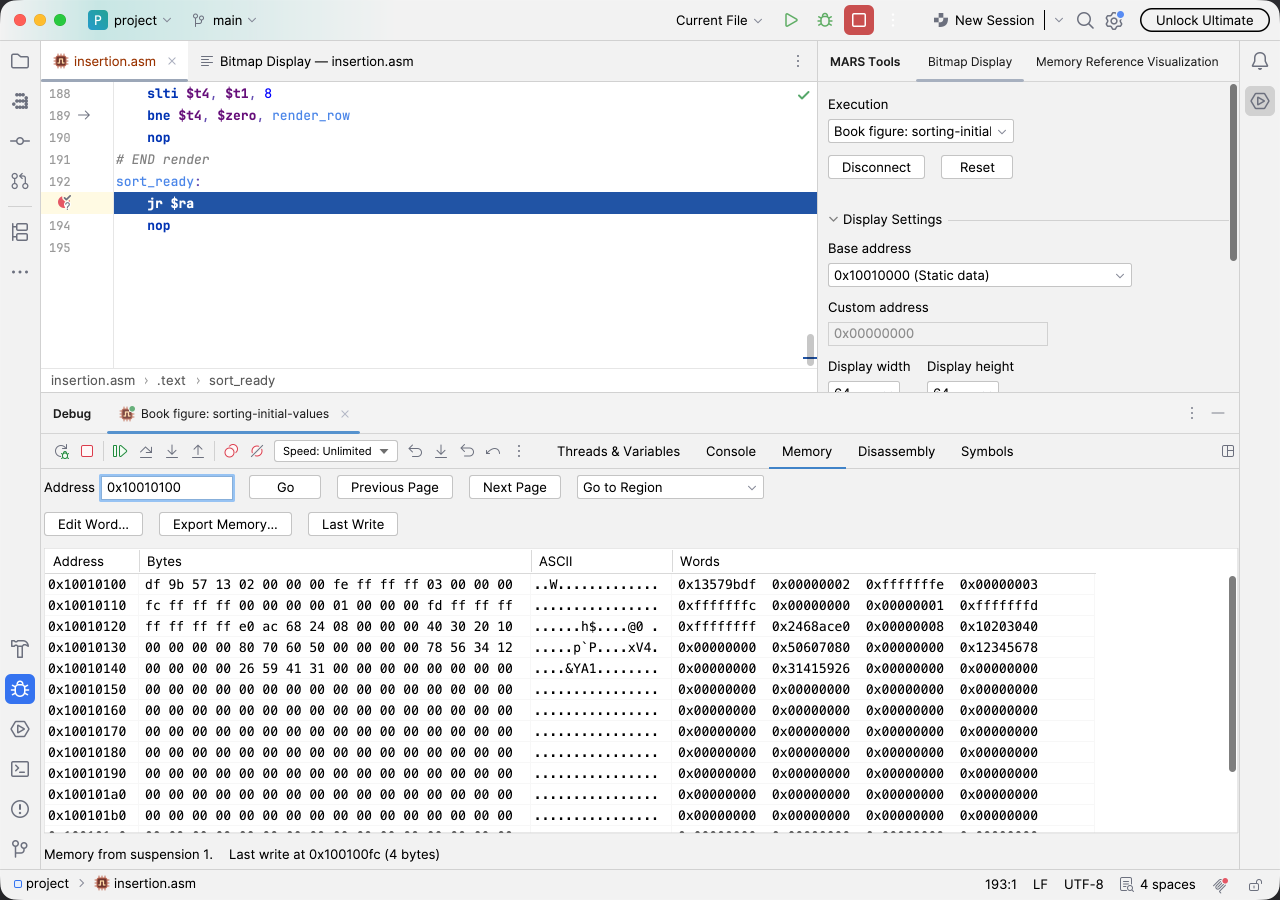
\includegraphics[artifact]{packages/009-sorting-visualizer/captures/f01-initial/values.png}}
  \sbox2{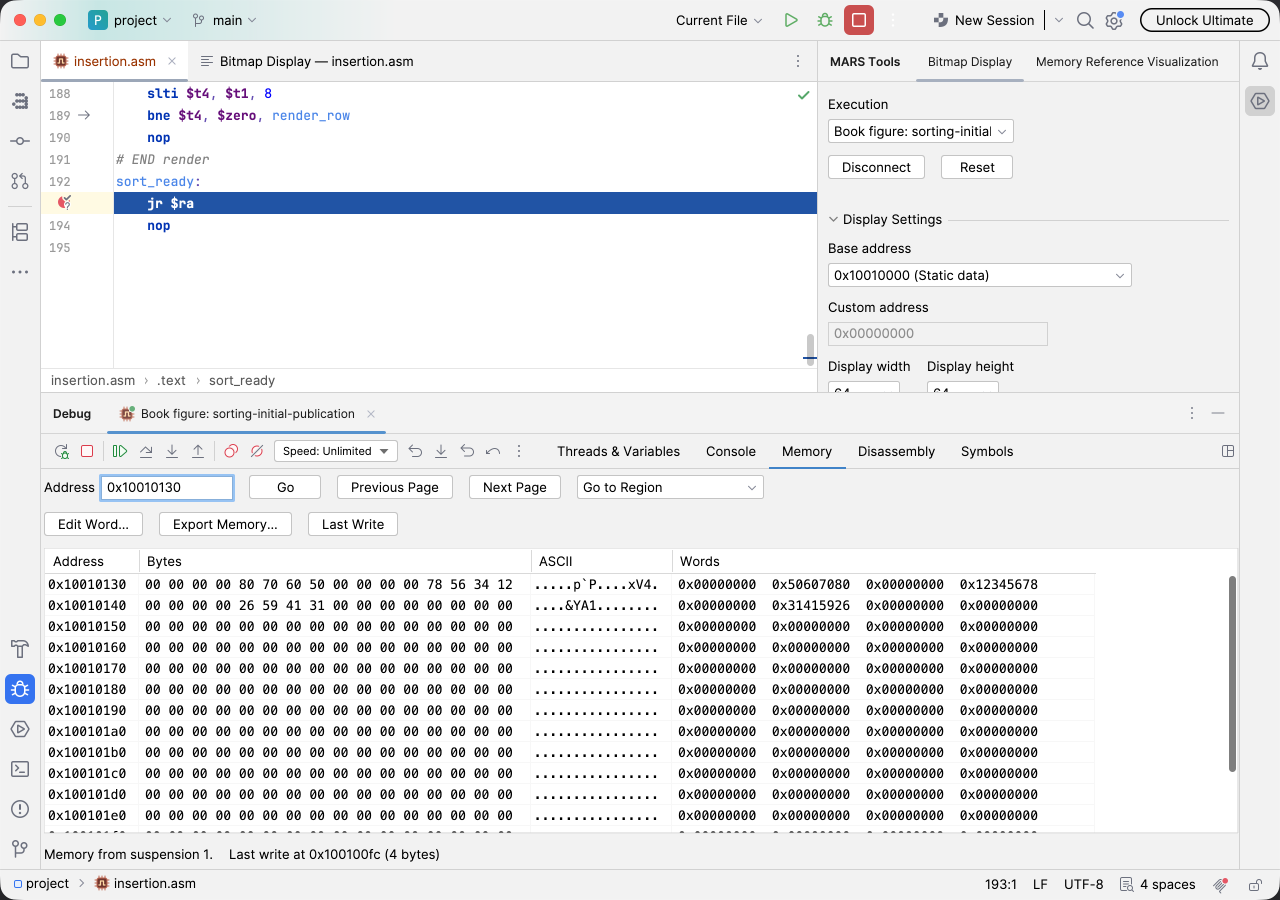
\includegraphics[artifact]{packages/009-sorting-visualizer/captures/f01-initial/publication.png}}
  \sbox4{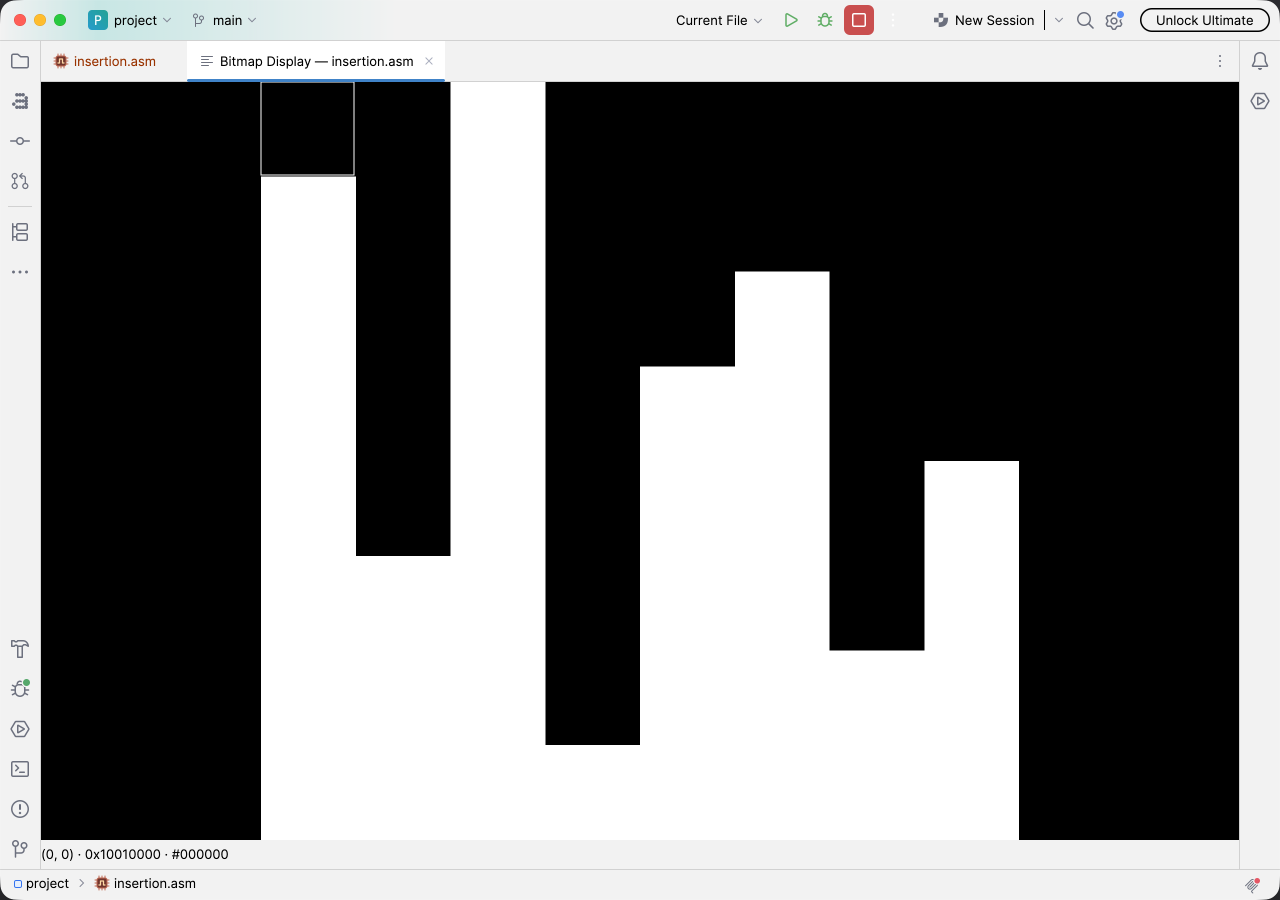
\includegraphics[artifact]{packages/009-sorting-visualizer/captures/f01-initial/bitmap.png}}
  \edef\MARSinitialsourceLeft{\the\dimexpr0.036718750\wd0\relax}
  \edef\MARSinitialsourceBottom{\the\dimexpr0.757777778\ht0\relax}
  \edef\MARSinitialsourceRight{\the\dimexpr0.611718750\wd0\relax}
  \edef\MARSinitialsourceTop{\the\dimexpr0.164444444\ht0\relax}
  \edef\MARSinitialstateLeft{\the\dimexpr0.034375000\wd0\relax}
  \edef\MARSinitialstateBottom{\the\dimexpr0.287777778\ht0\relax}
  \edef\MARSinitialstateRight{\the\dimexpr0.578906250\wd0\relax}
  \edef\MARSinitialstateTop{\the\dimexpr0.608888889\ht0\relax}
  \edef\MARSinitialmemoryLeft{\the\dimexpr0.034375000\wd2\relax}
  \edef\MARSinitialmemoryBottom{\the\dimexpr0.311111111\ht2\relax}
  \edef\MARSinitialmemoryRight{\the\dimexpr0.578906250\wd2\relax}
  \edef\MARSinitialmemoryTop{\the\dimexpr0.608888889\ht2\relax}
  \edef\MARSinitialplotLeft{\the\dimexpr0.203906250\wd4\relax}
  \edef\MARSinitialplotBottom{\the\dimexpr0.066666667\ht4\relax}
  \edef\MARSinitialplotRight{\the\dimexpr0.203906250\wd4\relax}
  \edef\MARSinitialplotTop{\the\dimexpr0.091111111\ht4\relax}
  \begin{tikzpicture}[alt={Four annotated details at the initial sort ready return boundary. The array is two, minus two, three, minus four, zero, one, minus three, minus one. The algorithm selector, phase and exchange count are zero. The eight white bar heights are seven, three, eight, one, five, six, two and four.}]
    \node[anchor=north west,inner sep=0,font=\small\bfseries] (source-title) at (6mm,0) {Next instruction: return from the renderer};
    \node[anchor=north west,inner sep=0] (source) at ([yshift=-1mm]source-title.south west) {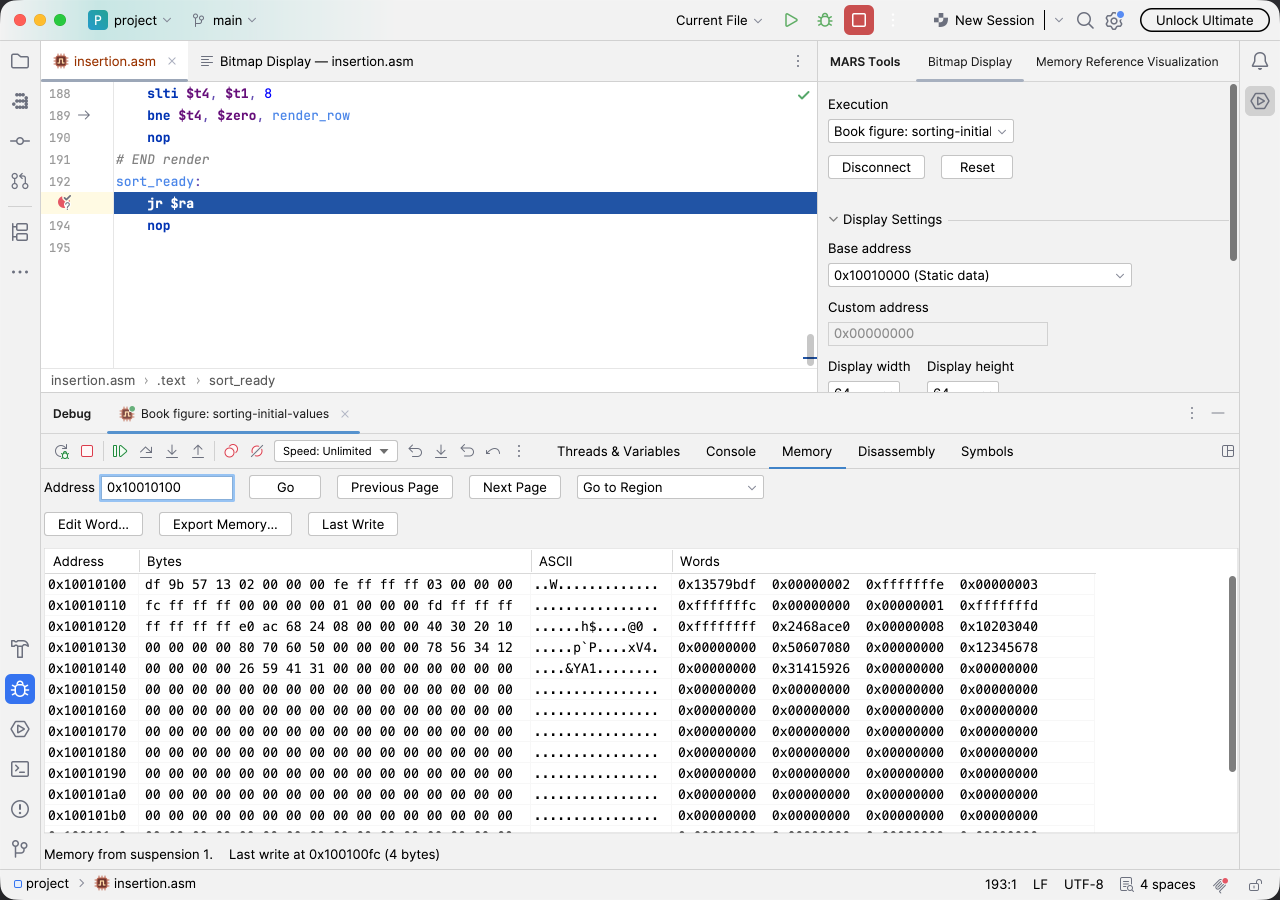
\includegraphics[width=0.7\linewidth,artifact,trim={\MARSinitialsourceLeft{} \MARSinitialsourceBottom{} \MARSinitialsourceRight{} \MARSinitialsourceTop{}},clip]{packages/009-sorting-visualizer/captures/f01-initial/values.png}};
    \begin{scope}[shift={(source.south west)},x={($(source.south east)-(source.south west)$)},y={($(source.north west)-(source.south west)$)}]
      \draw[black,line width=0.7pt] (0.153333333,0.057142857) rectangle (0.326666667,0.371428571);
      \node[draw=black,fill=white,circle,inner sep=1.5pt,font=\footnotesize] at ($(0.153333333,0.371428571)+(-3mm,0)$) {1};
    \end{scope}
    \node[anchor=north west,inner sep=0,font=\small\bfseries] (state-title) at ([yshift=-1mm]source.south west) {Signed array words and neighboring guards};
    \node[anchor=north west,inner sep=0] (state) at ([yshift=-1mm]state-title.south west) {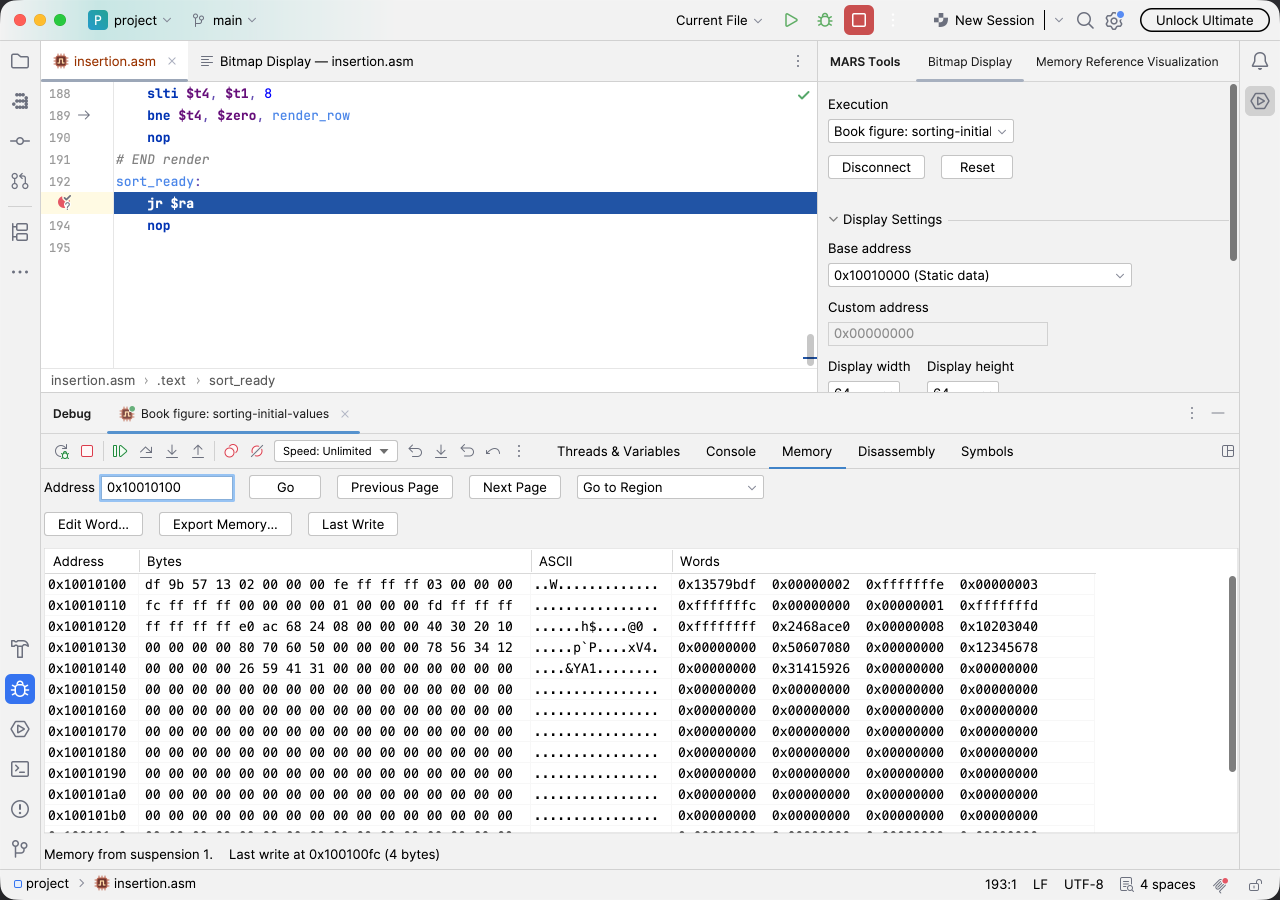
\includegraphics[width=0.78\linewidth,artifact,trim={\MARSinitialstateLeft{} \MARSinitialstateBottom{} \MARSinitialstateRight{} \MARSinitialstateTop{}},clip]{packages/009-sorting-visualizer/captures/f01-initial/values.png}};
    \begin{scope}[shift={(state.south west)},x={($(state.south east)-(state.south west)$)},y={($(state.north west)-(state.south west)$)}]
      \draw[black,line width=0.7pt] (0.191919192,0.043010753) rectangle (0.983838384,0.720430108);
      \node[draw=black,fill=white,circle,inner sep=1.5pt,font=\footnotesize] at ($(0.191919192,0.720430108)+(-3mm,0)$) {2};
    \end{scope}
    \node[anchor=north west,inner sep=0,font=\small\bfseries] (memory-title) at ([yshift=-1mm]state.south west) {Algorithm, phase and completed-exchange count};
    \node[anchor=north west,inner sep=0] (memory) at ([yshift=-1mm]memory-title.south west) {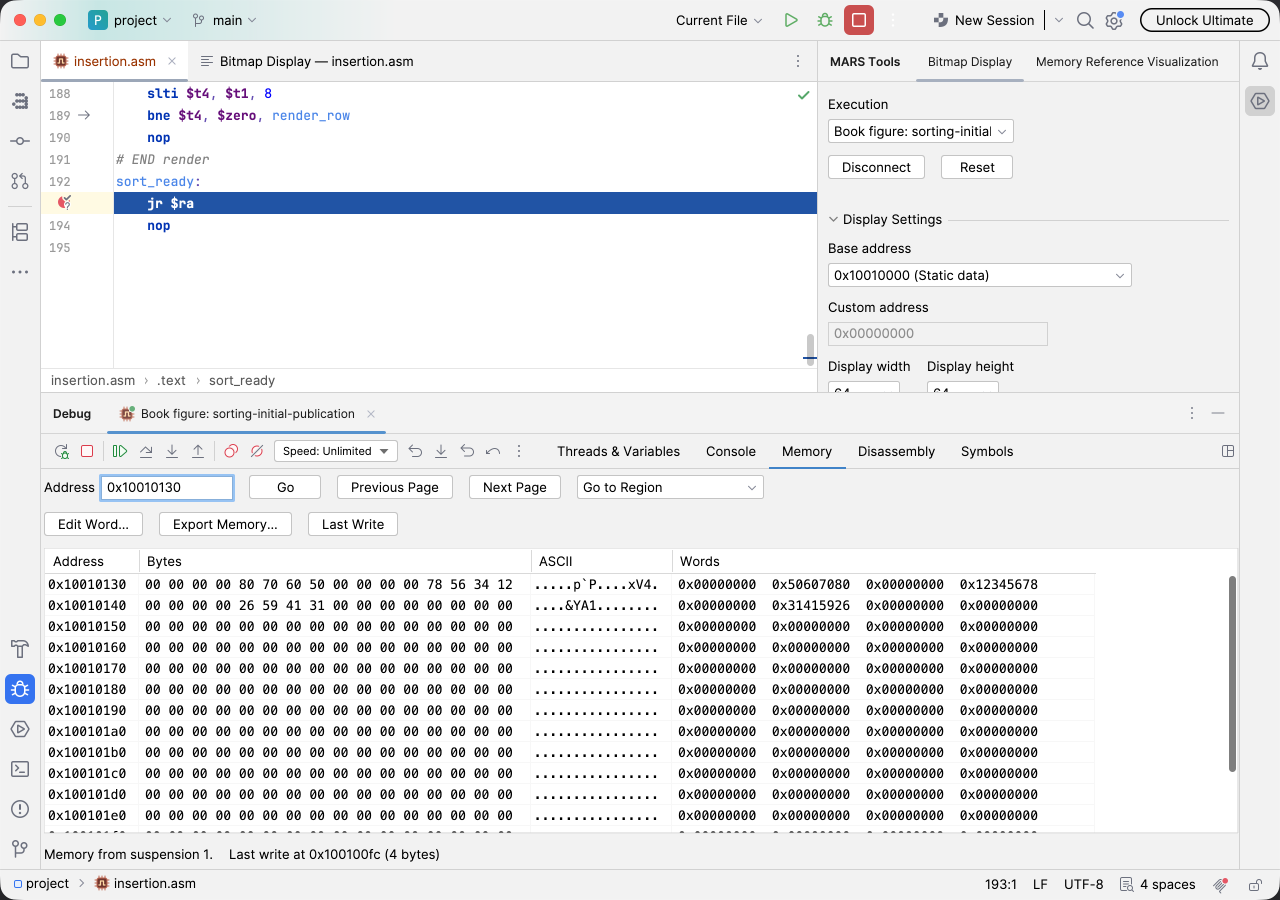
\includegraphics[width=0.78\linewidth,artifact,trim={\MARSinitialmemoryLeft{} \MARSinitialmemoryBottom{} \MARSinitialmemoryRight{} \MARSinitialmemoryTop{}},clip]{packages/009-sorting-visualizer/captures/f01-initial/publication.png}};
    \begin{scope}[shift={(memory.south west)},x={($(memory.south east)-(memory.south west)$)},y={($(memory.north west)-(memory.south west)$)}]
      \draw[black,line width=0.7pt] (0.191919192,0.055555556) rectangle (0.983838384,0.638888889);
      \node[draw=black,fill=white,circle,inner sep=1.5pt,font=\footnotesize] at ($(0.191919192,0.638888889)+(-3mm,0)$) {3};
    \end{scope}
    \node[anchor=north west,inner sep=0,font=\small\bfseries] (plot-title) at ([yshift=-1mm]memory.south west) {Complete published framebuffer};
    \node[anchor=north west,inner sep=0] (plot) at ([yshift=-1mm]plot-title.south west) {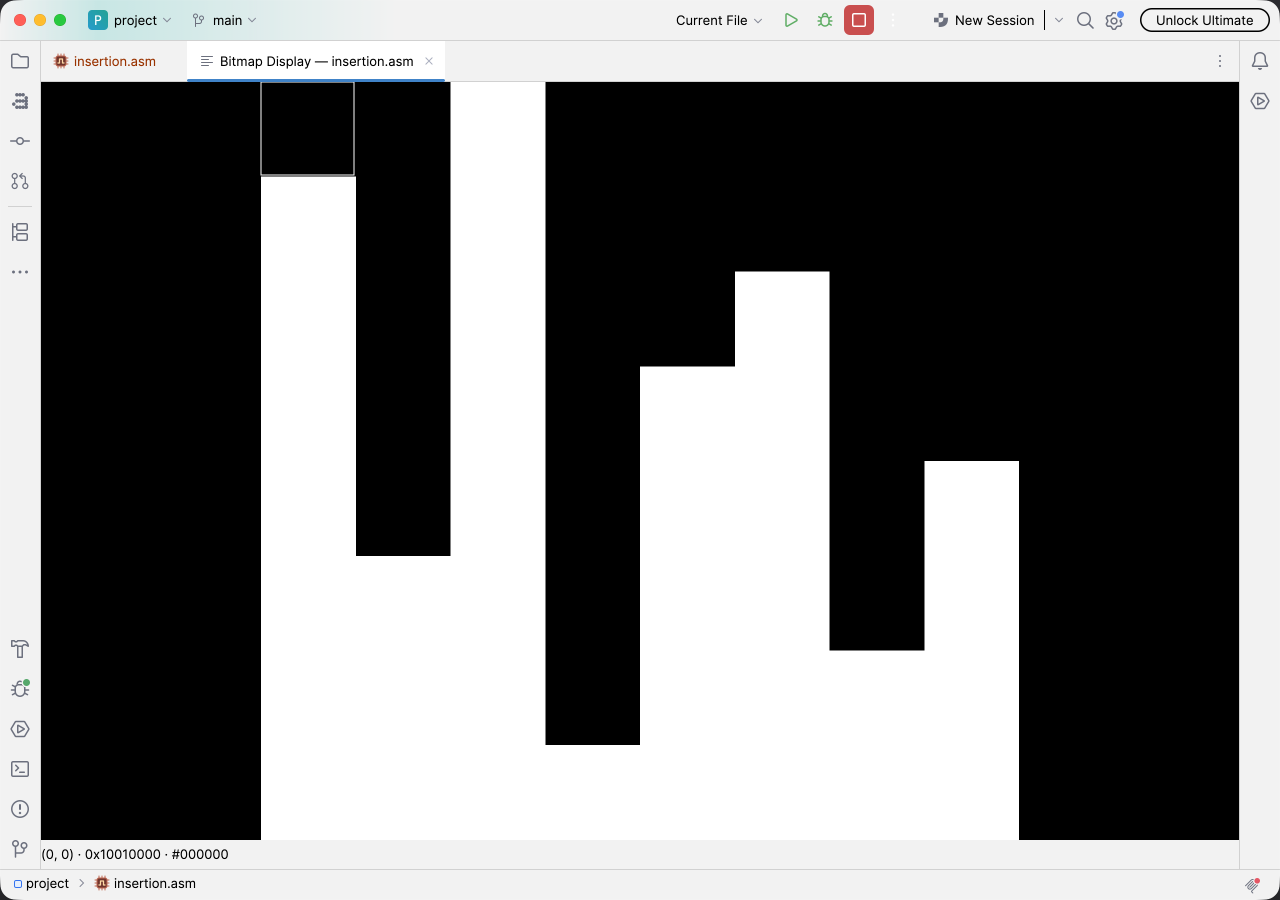
\includegraphics[width=0.24\linewidth,artifact,trim={\MARSinitialplotLeft{} \MARSinitialplotBottom{} \MARSinitialplotRight{} \MARSinitialplotTop{}},clip]{packages/009-sorting-visualizer/captures/f01-initial/bitmap.png}};
    \begin{scope}[shift={(plot.south west)},x={($(plot.south east)-(plot.south west)$)},y={($(plot.north west)-(plot.south west)$)}]
      \draw[black,line width=0.7pt] (0.000000000,0.000000000) rectangle (1.000000000,1.000000000);
      \node[draw=black,fill=white,circle,inner sep=1.5pt,font=\footnotesize] at ($(0.000000000,1.000000000)+(-3mm,0)$) {4};
      \foreach \c in {0,...,7} {\node[anchor=north,font=\scriptsize,inner sep=0] at ({(\c+0.5)/8},-0.035) {\c}; \node[anchor=east,font=\scriptsize,inner sep=0] at (-0.025,{1-(\c+0.5)/8}) {\c};}
      \node[anchor=north,font=\scriptsize,inner sep=0] at (0.5,-0.11) {$x$}; \node[anchor=east,font=\scriptsize,inner sep=0] at (-0.10,0.5) {$y$};
    \end{scope}
  \end{tikzpicture}
  \par\smallskip
  \begin{minipage}{\linewidth}
    \small
    \begin{enumerate}
      \item The blue \texttt{jr \$ra} is the next instruction. The initial renderer call has written all 64 pixel words but has not returned. The condition \texttt{\$s6 == 0} selects this initial publication before sorting begins.
      \item The eight values begin at \texttt{0x10010104}, after the framebuffer guard in the first displayed row. Read them as signed words: $[2,-2,3,-4,0,1,-3,-1]$. For example, bytes \texttt{fe ff ff ff} at \texttt{0x10010108} encode \texttt{0xfffffffe}, or $-2$. The array ends at \texttt{0x10010123}; the following guard and count are not array elements.
      \item At \texttt{0x10010130}, selector 0 chooses insertion sort. Phase at \texttt{0x10010138} is 0, and \texttt{swap\_count} at \texttt{0x10010140} is also 0. The intervening guard words are unchanged. These fields describe the complete frame at this return boundary.
      \item Column $x$ represents array element $x$, with height $v+5$. Thus 2 gives seven white cells and $-4$ gives one. The heights are $[7,3,8,1,5,6,2,4]$. Row 0 is at the top; the first white row is $3-v$. The thin outline in cell $(0,0)$ is the native selection marker.
    \end{enumerate}
  \end{minipage}
  \caption{The first complete frame displays the original signed array.}
  \label{capture:009-sorting-visualizer-f01-initial}
\end{figure}
\par
